\documentclass[10pt, letterpaper]{article}
        \usepackage[utf8]{inputenc}
        \usepackage[margin=1in]{geometry}
        \usepackage{fancyhdr}
        \usepackage{titling}
        \usepackage{enumitem}
        \usepackage{mathtools}
        \usepackage{amssymb}
        \usepackage{xfrac}
        \usepackage{booktabs}
        \usepackage{graphicx}
        \usepackage{wrapfig, blindtext}
        \usepackage{hyperref}
        \usepackage{enumerate}
        \usepackage{multicol}

        
        \setlength{\parindent}{0pt}

\title{Journal 2}
        \author{Sudhan Chitgopkar}
        \date{\today}
        
        % headers -- no need to change
        \pagestyle{fancy}
        \fancyhf{}
        \lhead{PFII}
        \chead{UGAMUNC XXVII}
        \rhead{\thedate}


\begin{document}

Dear Delegates, \\

It is with utmost pleasure to welcome you to the Permanent Forum on
Indigenous Issues (PFII). My name is Albert Chen, and I am so excited to
serve as your chair for UGA's 27\textsuperscript{th} Model United
Nations Conference. I am a current second-year from Marietta, Georgia
majoring in International Affairs, Finance, and International Business
with minors in Music and Chinese. In addition to Model UN, I am a
violist in UGA's Symphony Orchestra and a member of Apollo Business
Society. I am a huge Taylor Swift fan (stream any of her albums, I'm not
elitist), but I also appreciate the masterpiece that is Carly Rae
Jepsen's second studio album, Emotion. In my free time, I really enjoy
playing tennis, rock climbing, or hanging out with my friends. I am also
an avid watcher of the Bachelor \emph{and} the Bachelorette. Model UN
has played a huge part in shaping who I am today, and the UGA Model UN
team has given me a better community than I could ever ask for. I have
grown to love and value what Model UN can teach delegates: leadership,
teamwork, and public speaking. \\

I hope that you, the delegate, will compete to the best of your ability
and prepare adequately. Please note that this background guide is meant
to give you a foundation for further research, rather than an
all-encompassing reference for your preparation. That being said, I
would like to also note that this committee will at times discuss
politically sensitive topics. Thus, I hope that you will carry yourself
with the highest level of professionalism and debate respectfully and
responsibly. Additionally, as delegates of your country, I expect that
the scope of your position papers and your proposed strategies in debate
are in line with the views of your country. Delegates should consider
the history, politics, culture, and the demographics of the country
which they represent, even if you do not personally agree with these
views. The PFII seeks to put forth resolutions that address the three
important problems relating to the international community. \\

I would like to remind the delegates that each nation is equally
important in drafting resolutions, so please remember that when
preparing for the conference. I am specifically looking for cooperation
and efforts to give each nation a voice rather than one or two nations
leading a block. At the beginning of the conference, I will review
parliamentary procedure, but I urge you to review UGAMUNC rules and
procedures on our website:
\texttt{\href{https://www.ugamunc.com/}{{ugamunc.com}}}. If you have
any questions or concerns prior to the committee, my email is
\texttt{\href{mailto:azc81952@uga.edu}{{azc81952@uga.edu}}}. I am happy
to answer any and all questions you may have. I am looking forward to a
great committee and weekend! Please submit your completed position
papers (1 page per topic) to me by \textbf{11:59PM, January
29\textsuperscript{th},} and cite your sources using footnotes. I am
hoping to find specific, well thought out solutions to the topics listed
and any past action your country may have done. Thank you so much, and I
am looking forward to meeting you all! \\

Albert

\newpage
\tableofcontents
\newpage

\section{{What is the PFII?}}

The United Nations Permanent Forum on Indigenous Issues (PFII) is an
advisory body within the UN that reports to the UN's Economic and Social
Council (ECOSOC). PFII was founded in 2000 and deals with matters
concerning the rights of the world's indigenous peoples. ``Indigenous''
in this context means native, original, first people, and aboriginal
people. It is this committee's responsibility to provide expert advice
to ECOSOC about various topics under its purview; raise awareness of
activities related to indigenous issues within the UN system; and
disseminate information on indigenous issues.\footnote{``Permanent Forum
  on Indigenous Issues For Indigenous Peoples,'' accessed October 20,
  2020,
  https://www.un.org/development/desa/indigenouspeoples/about-us/permanent-forum-on-indigenous-issues.html.} \\

The PFII is composed of sixteen independent experts. Eight of these
members are nominated by Indigenous Peoples Organizations and the other
eight are nominated by governments. While PFII is a smaller committee
size, it still seeks to cover issues in all regions as the government
nominated experts are based on the five regional groupings normally used
in the UN\footnote{Ibid.} \\

It is vital to be aware that the PFII reports directly to ECOSOC and not
the UN General Assembly or UN Security Council. Also, please keep in
mind the central missions of providing expert advice and disseminating
information. \\

The PFII fills an important niche in the international community, giving
a voice to indigenous peoples who are largely ignored when selecting
government offices or representatives to the UN. Its focus on topics
that are largely ignored by other UN bodies makes it one of the few
lines of defense that indigenous groups have from losing their identity
to globalization and other countries' expansions. Because it is one of
the only bodies that adequately reports indigenous issues, it covers
multiple aspects of indigenous peoples, ranging from human rights
violations to economic issues. However, because no member of this
committee is a member of an indigenous group, be aware of what actions
your resolution may include. I look forward to seeing you debate these
multifaceted topics. \\

\newpage
\section{{Topic A: The Xinjiang Conflict}}

\subsection{Introduction:}

\begin{wrapfigure} {r}{0pt}
\centering
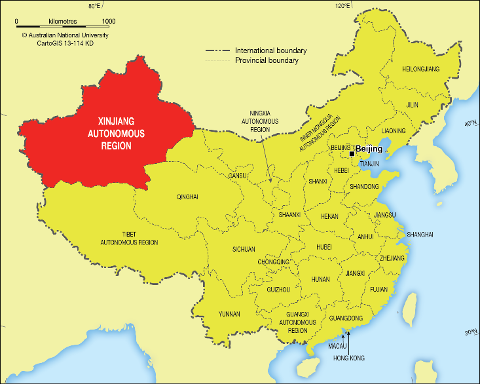
\includegraphics[width=3.332in,height=2.66667in]{Picture1.png} 
\caption{Xinjiang
Map\footnote{``Defense of the Republic of the Philippines,'' China's
  Uighur problem, accessed October 20, 2020,
  http://defenseph.net/drp/index.php?topic=121.0.}}
\end{wrapfigure}

The Xinjiang Uyghur Autonomous Region (XUAR) region (Figure 1) is in the
northwest corner of China with a majority Uyghur population. It is
China's largest province and provides several strategic advantages being
rich and natural resources and sharing borders with eight other
countries.\footnote{``Permanent Forum on Indigenous Issues For
  Indigenous Peoples,'' accessed October 20, 2020,
  https://www.un.org/development/desa/indigenouspeoples/about-us/permanent-forum-on-indigenous-issues.html.}
The Uyghur population established a kingdom in present-day north-central
Mongolia and are mentioned in Chinese records as early as the
3\textsuperscript{rd} century CE. In the 1950s, large populations of Han
Chinese began moving into the Xinjiang territory. Tensions rose between
the Uyghur and Han Chinese populations and escalated into protests and
disturbances. Violent incidents increased, and Chinese authorities began
responding with shootings, arrests, and jail sentences until 2017, when
the Chinese government set up cameras, checkpoints, and police patrols
in Uyghur-populated areas. The Chinese government has also reportedly
placed one million Uyghurs into indefinite detention into re-education centers. \footnote{``Uighur,'' Encyclopædia Britannica
  (Encyclopædia Britannica, inc.), accessed October 20, 2020,
  https://www.britannica.com/topic/Uighur.} \\

This committee is concerned with the potential human rights violations
against the Uyghurs that may be occurring within the Xinjiang Conflict.
The committee will need to balance national sovereignty rights alongside
the responsibility to protect indigenous populations. \\

\subsection{Topic Background}

The Uyghur population in the Xinjiang province is a remainder of the
Uyghur Empire from the eighth century. The Uyghur majority is largely
Sunni Muslim, a far cry from the non-religious Han Chinese. For a brief
period after 1864, Xinjiang was to break away from China while it was
weakened by other conflicts. However, Chinese control was reasserted in
1877. The Chinese Government put heavy taxes on the Uyghur populations
to finance Han Chinese migration and settlement into the best land in
the province.\footnote{United Nations High Commissioner for Refugees,
  ``World Directory of Minorities and Indigenous Peoples - China :
  Uyghurs,'' Refworld, accessed October 20, 2020,
  https://www.refworld.org/docid/49749d3c4b.html.} \\

In 1949, Uyghur leaders were invited to speak with Mao Zedong about
Uyghur independence which was promised in exchange for them supporting
the Communists in the civil war, but the plane crashed on its way to
Beijing. The region later took shape on October 1, 1955 as the Xinjiang
Uyghur Autonomous Region. However, tensions continued to rise as Chinese
Communist officials began to favor the Han Chinese.\footnote{United
  Nations High Commissioner for Refugees, ``World Directory of
  Minorities and Indigenous Peoples - China : Uyghurs,'' Refworld,
  accessed October 20, 2020,
  https://www.refworld.org/docid/49749d3c4b.html.} The Han Chinese are
said to be given the best jobs the majority do well
economically.\footnote{``Why Is There Tension between China and the
  Uighurs?,'' BBC News (BBC, September 26, 2014),
  https://www.bbc.com/news/world-asia-china-26414014.} \\

In 1962, 60,000 to 100,000 Uyghurs fled the country to avoid repression
and famine from the Great Leap Forward. The Chinese Government also
began imposing restrictions on Uyghur religious and cultural practices
as well as began seizing land. Student demonstrations and riots arose in
the 1980s to oppose the Han migration. In 1990, the Baren Township riot
resulted in at least 50 people being killed. These protests further
escalated into bombing incidents as well as attacks against Chinese
soldiers and officials.\footnote{United Nations High Commissioner for
  Refugees, ``World Directory of Minorities and Indigenous Peoples -
  China : Uyghurs,'' Refworld, accessed October 20, 2020,
  https://www.refworld.org/docid/49749d3c4b.html.} \\

After the Chinese execution of 30 suspected separatists, large
demonstrations occurred in February 1997. Chinese media called these
demonstrations ``violent riots''\footnote{``Xinjiang to Intensify
  Crackdown on Separatists,'' Global Edition, accessed October 20, 2020,
  http://www.chinadaily.com.cn/en/doc/2001-10/25/content\_90592.htm.}
whereas western news outlets characterized them as peaceful.\footnote{``
  CHINA: REMEMBER THE GULJA MASSACRE? CHINA'S CRACKDOWN ON PEACEFUL
  PROTESTERS,'' Amnesty International, 2007,
  https://www.amnesty.org/en/documents/asa17/002/2007/en/.} This
culminated in the Ghulja Incident, where the Chinese army crackdown led
to at least nine deaths.\footnote{``China: Human Rights Concerns in
  Xinjiang,'' China: Human Rights Concerns in Xinjiang (Human Rights
  Watch Backgrounder, October 17, 2001), 2001,
  https://www.hrw.org/legacy/backgrounder/asia/china-bck1017.htm.}
Conflicts have continued to escalate, and Uyghur separatists claimed
responsibilities for bus bombings in Beijing.\footnote{Rémi Castets,
  ``The Uyghurs in Xinjiang -- The Malaise Grows,'' China Perspectives
  (French Centre for Research on Contemporary China, July 31, 2006),
  https://journals.openedition.org/chinaperspectives/648.} \\

Following China's secondary crackdown before the 2008 Beijing Olympics,
the number of violent incidents and attacks have only increased,
including a plane hijacking in 2012, a knife attack in 2013, and a
bombing in 2014. China has blamed the East Turkestan Islamic Movement
(ETIM) for multiple violent incidents, a group which the United States
classifies as ``the most militant of the ethnic Uyghur separatist
groups.''\footnote{``Why Is There Tension between China and the
  Uighurs?,'' BBC News (BBC, September 26, 2014),
  https://www.bbc.com/news/world-asia-china-26414014.} \\

In 2017, President Xi Jinping set up Xinjiang Re-education camps to
indoctrinate Uyghurs and other Muslims as part of a ``people's war on
terror'' The Chinese Government has also began to ``treat expressions of
Uyghur identity\ldots{} as one of the three evil forces''. There is very
little information about these facilities, and the number of people held
in them varies between 2000 to 5000.\footnote{``China: Free Xinjiang
  'Political Education' Detainees,'' Human Rights Watch, October 20,
  2020,
  https://www.hrw.org/news/2017/09/10/china-free-xinjiang-political-education-detainees.}
Detainees are not released until total ideological transformation. This
includes renouncement of their religion, forced learning of the Mandarin
language, and promoting repentance.\footnote{``Data Leak Reveals How
  China 'Brainwashes' Uighurs in Prison Camps,'' BBC News (BBC, November
  24, 2019), https://www.bbc.com/news/world-asia-china-50511063.} There
is no official knowledge on other punishments being used. \\

\subsection{UN Action}

There has been little official action by the UN on this topic until
recently. The establishment of the political re-education centers has
made the UN more aware of the Xinjiang Conflict. Nearly two dozen
countries confronted China at the United Nations in October 2019. A
group of 23 countries released a statement to the UN General Assembly
the Third,condemning the actions of the Chinese government, but nearly
50 countries supporting China sought to ``commend China's remarkable
achievements in the field of human rights.''\footnote{``Countries Blast
  China at UN Over Xinjiang Abuses,'' Human Rights Watch, October 20,
  2020,
  https://www.hrw.org/news/2019/10/30/countries-blast-china-un-over-xinjiang-abuses.}
Because this issue was only brought to the General Assembly in late
2019, there has been little opportunity for further debate of this
topic. It is up to this committee to debate and determine the UNPFII
stance on the Xinjiang Conflict. \\

\subsection{Current Situation}

China has continually justified its stance and its actions through its
euphemistic naming of its re-education centers and saying the violent
actions of the ETIM warrant an equally violent response. Testimonies
from survivors paint these camps as internment camps or prisons. This is
especially of concern as the COVID-19 pandemic still rages on. \\

Without any proper protective gear, hygienic facilities, or social
distancing, COVID-19 could easily tear through the Uyghur communities.
There has been virtually no information on the real figure of COVID-19
in Uyghur communities.\footnote{Vaishnavi C Chaudhry, ``The Impact of
  COVID-19 on Uighur Muslims: An Ignored Crisis,'' LSE Human Rights,
  July 13, 2020,
  https://blogs.lse.ac.uk/humanrights/2020/04/23/the-impact-of-covid-19-on-uighur-muslims-an-ignored-crisis/.} \\

The harsh treatment of the Uyghurs has not stopped, but only escalated
in recent years. However, the number of violent attacks from Uyghur
separatist groups has dropped to almost zero. The Permanent Forum on
Indigenous Issues must carefully discuss and debate the issues at hand.
Violence should be reduced as much as possible through a resolution that
is passed in committee. \\

\subsection{Relevant Vocabulary/Notes}

\begin{itemize}
\item
  
  \textbf{Uyghur/Uighur:} Both spellings are accepted, but for this committee and
  conference, please use ``Uyghur''.\footnote{``Uighur,'' Encyclopædia
    Britannica (Encyclopædia Britannica, inc.), accessed October 20,
    2020, https://www.britannica.com/topic/Uighur.} There is contention
  on whether or not the Uyghurs are truly indigenous. The final decision
  will be up to the committee, but for the sake of opening debate, we
  will assume that this topic falls under the purview of the PFII.
  
\item
  
 \textbf{ Responsibility to Protect:} An international norm that affirms the
  responsibility of states to protect populations from genocide, war
  crimes, and crimes against humanity.\footnote{``The Responsibility to
    Protect,'' United Nations (United Nations), accessed October 20,
    2020,
    https://www.un.org/en/chronicle/article/responsibility-protect.}
  
\item
  
  \textbf{Uyghur-Chinese Conflict and Xinjiang Conflict are synonymous.}
  
\end{itemize}

\subsection{Questions to Consider:}

\begin{itemize}
\item
  
  Do the violent attacks from Uyghur separatist groups count as domestic
  terrorism/ terrorist attacks?
  
\item
  
  Has China violated human rights by establishing their re-education
  centers?
  
\item
  
  Is the violent response by Chinese Authorities to the violent protests
  reasonable? Reflect upon your own country's history in dealing with
  violent protests.
  
\item
  
  Should some groups of the Uyghur separatist movement be punished for
  their violent actions?
  
\item
  
  What is the best way to de-escalate the conflict and negotiate peace
  between the two parties? Consider the 1949 plane crash.
  
\end{itemize}

\subsection{Suggested Readings:}

\begin{itemize}
\item
  
  
  \texttt{\href{https://www.cfr.org/backgrounder/chinas-repression-uighurs-xinjiang}{{A timeline and good overview of the Uyghur Crisis.}}}
  
\item
  
  
 \texttt{ \href{https://fsi.stanford.edu/news/human-rights-crisis-xinjiang-uyghur-autonomous-region}{{A summary of a Stanford Panel on the Xinjiang Crisis}}}
  
\item
  
  
  \texttt{\href{https://thediplomat.com/2018/11/xinjiang-detention-camp-or-vocational-center-is-china-calling-a-deer-a-horse/}{{More info on the Political Re-education Centers}}}
  
\item
  
  \texttt{\href{https://www.nytimes.com/2020/07/19/world/asia/china-mask-forced-labor.html}{{Article on forced Uyghur Labor}}}
  
\item
  
  
  \texttt{\href{https://www.independent.co.uk/news/world/asia/china-re-education-muslims-ramadan-xinjiang-eat-pork-alcohol-communist-xi-jinping-a8357966.html}{Article on some extreme punishments being issued}}
  
\end{itemize}

\newpage
\section{{Topic B: The Kurdish Stateless Nation}}

\subsection{Introduction} 
\begin{wrapfigure} {r} {0pt}
\centering
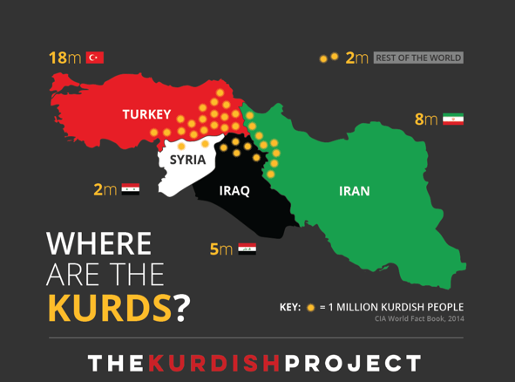
\includegraphics[scale = 0.75]{Picture2.png} 
\caption{The Kurdish Project Map\footnote{``Kurdistan Map.'' \emph{The Kurdish Project},
  thekurdishproject.org/kurdistan-map/.}}
\end{wrapfigure}


The Kurdish people are a stateless ethnic group of approximately 30
million located in parts of northern Syria, northwestern Iran, eastern
Turkey and northern Iraq (Figure 2). On a global scale, the group is
known for its cultural diversity that spreads across the four states it
inhabits. However, the Kurds have been persecuted as they are an ethnic
minority in the states of which they reside. Over the years, tens of
thousands of Kurds have been killed in genocides in Syria, faced
political oppression in Iraq, and currently are at odds with the Turkish
government. Since before World War I, the Kurds have been pushing for
the declaration of autonomy and statehood, with little to no conclusion
in sight. In addition to numerous refugees and destruction of civilian
lives, these conflicts are putting Kurdish culture at risk. The issues
of preserving the history of this ethnic group and addressing their
countless calls for independence, while also keeping the lives of the
displaced people safe must be addressed by this committee. \\



\subsection{Topic Background}

The Kurds originated between the contending empires of the Ottomans and
the Persians for centuries.\footnote{``THE ANCIENT ROOTS OF THE KURDS.''
  \emph{TIME SIFTERS ARCHAEOLOGY SOCIETY}, 31 Mar. 2016,
  www.timesifters.org/the-ancient-roots-of-the-kurds/.} Though the two
empires were divided by the natural barrier of the Zagros Mountains, the
Kurds had access to both and thus formed their own distinct language,
history and culture. After assisting the Ottomans in defeating the
Persians, the Kurds were offered self-governance in the region for
approximately 300 years until the Kurds asked for full independence and
were rejected.\footnote{Ibid.} Following World War 1, the Treaty of
Sevres both ended the Ottoman Empire and proposed an independent Kurdish
State. This proposition was also rejected, and the Kurdish people were
given some limited autonomy in the states of Turkey, Iran, Iraq, and
Syria.\footnote{``Timeline: The Kurds' Quest for Independence.''
  \emph{Council on Foreign Relations}, Council on Foreign Relations,
  www.cfr.org/timeline/kurds-quest-independence.} \\

About half of the Kurdish population lives in Turkey, where Kurdish
culture and political actions are silenced by the Turkish government and
with violent attempts to claim Kurdish equality in the
nation.\footnote{\emph{The Kurds in Turkey},
  fas.org/asmp/profiles/turkey\_background\_kurds.htm.} This has led to
the development of a separatist movement in the state that, while not
fully supported by all Turkish Kurds, has gained some popularity in the
region. Violence from this group's conflict with the Turkish government
has subsequently created nearly 2 million refugees in the
area.\footnote{Ibid.} Kurds living in the Persian Empire now live in
modern day Iran where the Iranian government has been less aggressive to
the Kurds, however they are still pushing for inclusion in the political
system. Numerous opposition groups have formed in Iran, such as the
Democratic Party of Iranian Kurdistan (PDKI) and the Kurdistan Free Life
Party (PJAK), who are using force against the Islamic Republic of
Iran.\footnote{Crahan, Garrett Nada and Caitlin. ``Iran's Troubled
  Provinces: Kurdistan.'' \emph{The Iran Primer},
  iranprimer.usip.org/blog/2020/sep/08/iran\%E2\%80\%99s-troubled-provinces-kurdistan.}
The state of Iraq initially showed more willingness to provide autonomy
for the Kurds, yet this was reversed as a consequence of the US-Iraqi
conflict. In 1988 the Iraqi Kurds faced a mass genocide led by Saddam
Hussein that killed tens of thousands and increased tensions in the
region.\footnote{``Timeline: The Kurds' Quest for Independence.''
  \emph{Council on Foreign Relations}, Council on Foreign Relations,
  www.cfr.org/timeline/kurds-quest-independence.} Later in 2003, the
Kurds supported the United States in overthrowing Hussein, and in 2005,
were recognized as an autonomous region within Iraq.\footnote{``Iraq's
  Constitution of 2005.'' \emph{Constitute},
  www.constituteproject.org/constitution/Iraq\_2005.pdf?lang=en.} This
changed however when President Trump pulled U.S. forces out of the area
as tensions redeveloped between the Iraqi government and the
Kurds.\footnote{``Timeline: The Kurds' Quest for Independence.''
  \emph{Council on Foreign Relations}, Council on Foreign Relations,
  www.cfr.org/timeline/kurds-quest-independence.} The instability that
faces the Kurds in each region they inhabit leaves the group calling for
independence; a call which has been overlooked for centuries. \\

\subsection{UN Action:}

In 2004, the UN High Commissioner for Refugees (UNHCR) called attention
to the Iranian Kurds fleeing their homeland due to the upset brought on
by the Iraqi War.\footnote{``UN Appeals for Resettlement of Stranded
  Kurd Refugees 18 Months after Iraq War  UN
  News.'' \emph{United Nations}, United Nations,
  news.un.org/en/story/2004/12/123252-un-appeals-resettlement-stranded-kurd-refugees-18-months-after-iraq-war.}
This committee proposed resettlement of the Kurdish refugees to nations
including Australia, the United States, and some Scandinavian countries,
however these requests remained pending, and the situation has only
escalated from there.\footnote{Ibid.} Later in 2017, the UN Assistance
Mission for Iraq spoke in opposition of the violence occurring to the
political offices in the portion of Kurdistan in Iraq. The mission
addressed the Kurds' call for peace and paired it with the Iraqi
government's requests for de-escalation and legal order.\footnote{``News
  in Brief 30 October 2017 (PM) \textbar{} \textbar{} UN News.''
  \emph{United Nations}, United Nations,
  news.un.org/en/audio/2017/10/635242.} The situation was left with the
region being monitored as the Iraqi government suspended military
operations for the time being. Most recently, the UNHCR has reported
tens of thousands of refugees fleeing the violence of the Syrian
conflict in 2019. When addressing the UN Security Council, US Ambassador
Kelly Craft declared that Turkey bears responsibility for protecting the
Kurdish people and other minorities.\footnote{``De-Escalation of Turkish
  Military Operation in Northern Syria 'Absolutely Essential' \textbar{}
  \textbar{} UN News.'' \emph{United Nations}, United Nations,
  news.un.org/en/story/2019/10/1049021.} Turkey deems the Kurdish
fighters that have been supporting the United States as terrorists, thus
this poses many issues regarding their willingness to protect the ethnic
group's interest. The heavily debated issue of Kurdish independence and
at what levels that can be granted, allows opportunity for meaningful
resolutions to be developed in this committee. \\

\subsection{Current Situation}

The relationship between the Turkish government and the Kurds has been
tumultuous for years, but in 2019 it escalated. On October 6, 2019,
President Trump pulled U.S. troops out of Northern Syria which created a
domino effect of power struggles that ultimately allowed for Turkey to
gain control of the border area. The state established a 5000 sq. km
buffer zone that prohibits the presence of Kurdish people.\footnote{Vanessa
  BairdVanessa Baird lived and worked as a journalist in Peru during the
  tumultuous mid-1980s, et al. ``Betrayed Again.'' \emph{New
  Internationalist}, 6 July 2020,
  newint.org/features/2020/06/11/big-story-kurds-betrayed-again.} Turkey
has shown little willingness to give the Kurds autonomy in the past and
the Kurds face even more destruction of their culture and identity in
this state of violence. \\

Even with the onset of Covid-19 in the past six months, Turkey has
maintained its position against the Kurds. Because of the pandemic, the
United Nations called for a ceasefire with Turkish forces, yet they
continued their attacks on Northern Syria and have begun restricting
crucial resources from refugee camps that house many Kurdish
people.\footnote{Ibid.} Remaining Kurds in the area are also suffering
greatly at the hands of the Turkish government, with targeted violence
to their businesses and homes and even the people themselves. \\

Historically, Kurdish requests for independence have resulted in further
conflicts and violence. On the other hand, remaining internally
displaced threatens the preservation of the Kurdish culture, language,
and history. The Permanent Forum on Indigenous Issues values both the
preservation of this indigenous culture while also attempting to keep as
much peace in the area as possible. Both of these values should be
looked at extensively when writing a resolution. \\

\subsection{Vocabulary}

\begin{itemize}
\item
  
  \textbf{Treaty of Sevres}: A pact between the allied powers and
  Ottoman Turkey that proposed the first Kurdish state and the
  dissolvement of the Ottoman Empire. The treaty was not accepted by
  Turkish nationals and is some of the first official documentation of
  the first Turkish-Kurdish opposition.
  
\item
  
  \textbf{UN Assistance Mission for Iraq}: A UN establishment formed for
  the purposes of forming a political dialogue between Iraq and
  neighboring states as well as monitoring social and humanitarian
  issues involving the Iraqi state.
  
\end{itemize}

\subsection{Questions to Consider}

\begin{itemize}
\item
  
  Consider the long history of the Kurds in Turkey. How can your country
  provide an approach that protects the civilians on both sides of this
  conflict?
  
\item
  
  What are some solutions that can preserve Kurdish culture without
  immediately declaring statehood?
  
\item
  
  Consider the official qualifications for statehood. Is it likely that
  the Kurds can gain independence and become a state in the near future?
  
\item
  
  How might foreign involvement from outside of this region affect the
  situation (i.e. U.S troops in Syria)?
  
\item
  
  What are the efforts your state can take to maintain peace in this
  region?
  
\item
  
  Consider the conflicts the Kurds have had in states other than Turkey
  (Iraq, Iran, Syria). How might these relations affect your country's
  proposed solutions?
  
\end{itemize}

\subsection{Suggested Readings}

\begin{itemize}
\item
  
  
  \texttt{\href{https://thekurdishproject.org/}{Thorough explanation of the Kurdish state}}
  
\item
  
  
  \texttt{\href{https://www.cfr.org/timeline/kurds-quest-independence}{{Timeline of Kurdish history}}}
  
\item
  
  \texttt{
  \href{https://www.culturalsurvival.org/publications/cultural-survival-quarterly/kurdish-repression-turkey}{{Kurds in Turkey}}}
  
\item
  
  
  \texttt{\href{https://www.crisisgroup.org/middle-east-north-africa/gulf-and-arabian-peninsula/iraq/kurds-divided-future}{{Examines the Kurds relations with each state it inhabits}}}
  
\end{itemize}

\newpage
\section{{Topic C: Achieving SDGs within Indigenous
Populations}}

\subsection{Introduction}

The Sustainable Development Goals (SDGs) are 17 goals that were outlined
by the United Nations in 2015 that will lead to prosperity for the
international community by 2030. These goals include targets like no
poverty, gender equality, but also climate action, and life on land.
Indigenous peoples are mentioned 6 times in the SDGs specifically in
Goal 2: Zero Hunger, and Goal 4: Quality Education.\footnote{``THE 17
  GOALS \textbar{} Sustainable Development,'' United Nations (United
  Nations), accessed October 20, 2020, https://sdgs.un.org/goals.}
However, the issue of achieving SDGs within Indigenous populations
applies to all goals. \\

Lack of infrastructure, systematic discrimination, and lack of ability
to self-govern all prove to be barriers to achieving SDGs within
indigenous populations. There is also the additional problem of certain
cultural values conflicting against some indicators in the SDGs.
Overall, the committee must balance between preserving cultural values,
implementing SDGs, and behaving non-colonially when writing resolutions. \\

\subsection{Topic Background}

Indigenous peoples are a small proportion of the world's population but
represent an irreplaceable population segment. However, despite living
in resource rich areas, indigenous populations are consistently poor.
Despite only being 5\% of the world's population, indigenous populations
account for 15\% of the world's poor. Because indigenous communities
have been forced off their land for either resource extraction or
conservation efforts, their most valuable asset is unusable to
them.\footnote{``The Challenges We Face,'' FirstPeoples.org - The
  Challenges We Face, accessed October 20, 2020,
  http://www.firstpeoples.org/the-challenges-we-face.htm.} SDG 1 is no
poverty, but the road to achieving that goal is blocked by systematic
discrimination and seizing of rights. \\

Another significant issue that hinders the achievement of SDGs is the
lack of government recognition from foreign states. Because few
countries recognize indigenous peoples as legitimate groups, they are
excluded from political forums to defend their rights.\footnote{Ibid.}
Without their involvement in these forums, few bodies are even aware of
what indigenous populations need to help achieve the SDGs. In relation
to SDG 8 (Economic Growth and Decent Work), indigenous representatives
have stressed that recognition and protection of their traditional
occupations is vital \footnote{``Indigenous World 2020: The Sustainable
  Development Goals (SDGs) and Indigenous Peoples,'' IWGIA, accessed
  October 20, 2020,
  https://www.iwgia.org/en/ip-i-iw/3658-iw-2020-sdgs.html.}, but there
has been very little action from states to respond to their requests. \\

\begin{wrapfigure} {r} {0pt}
\centering
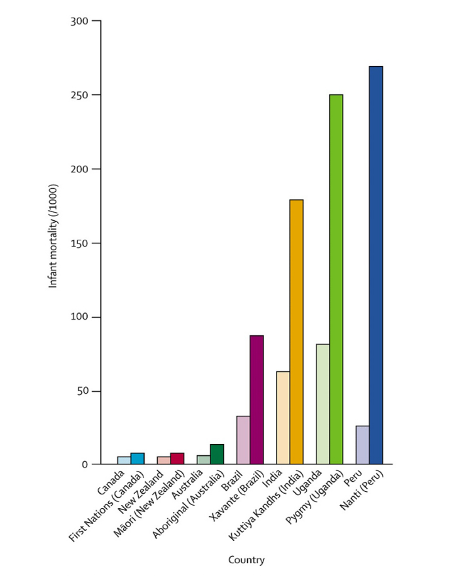
\includegraphics[width=3.20903in,height=2.75in]{Picture3.png} 
  \caption{Indigenous community infant mortality\footnote{``The
  Challenges We Face,'' FirstPeoples.org - The Challenges We Face,
  accessed October 20, 2020,
  http://www.firstpeoples.org/the-challenges-we-face.htm.}}
\end{wrapfigure}

The 2019 Global Sustainable Development Report (GSDR) explicitly
referenced indigenous peoples when saying that the world is not on track
for achieving the 2030 agenda. It highlighted ``continued discrimination
and exclusion from political and economic power'' as a major reason for
the lack of progress within indigenous populations.\footnote{Ibid.} \\

Compounding upon bureaucratic difficulties, many SDGs such as 13
(Climate Change) and 3 (Good Health) require technological capacity that
many indigenous populations are unable to afford.\footnote{Ibid.}
COVID-19 has highlighted weaknesses in the public health systems of
developed nations. Many indigenous populations that inhabit remote areas
do not have access to medical technologies that can save lives. As a
result, infant mortality is abnormally high within indigenous
populations compared to their country of residence (Figure 3). \\



Additionally, the culture of many indigenous populations may not be
conducive to achieving an SDG. If the culture or tradition has strict
gender roles, the more modern definition of gender equality may not be
accepted. This becomes an issue with cultural loss and forced
assimilation. If indigenous populations do not wish to achieve an SDG,
or only wish to work towards part of it, should they be given the
autonomy to follow their culture and tradition?

\subsection{UN Action}

The UN has already stated that all Sustainable Goals are relevant to
indigenous peoples. However, it also admits that the SDGs lack cultural
sensitivity.\footnote{``Indigenous Peoples and the 2030 Agenda,''
  \emph{Indigenous Peoples and the 2030 Agenda} (UN Permanent Forum on
  Indigenous Issues, n.d.),
  https://www.un.org/development/desa/indigenouspeoples/wp-content/uploads/sites/19/2016/10/Short-flyer\_UNPFII-Substantive-Inputs-2017.pdf}
There have been very few resolutions that address the lack of cultural
sensitivity already mentioned. However, the UN has continued broadening
its metrics for certain SDGs so that they are more applicable to
indigenous populations. The PFII is actively engaged in the SDG agenda
and ensuring that indigenous rights are being considered.\footnote{``The
  Permanent Forum and the 2030 Agenda For Indigenous Peoples,'' United
  Nations (United Nations), accessed October 20, 2020,
  https://www.un.org/development/desa/indigenouspeoples/focus-areas/post-2015-agenda/the-sustainable-development-goals-sdgs-and-indigenous/recommendations.html.}
Because the PFII puts considerable input to ECOSOC, this committee has
significant influence over the direction of the SDGs. \\

\subsection{Current Situation}

The SDGs have ``acknowledged that there can be no truly sustainable
development without protecting traditional knowledge and territories of
indigenous peoples.'' Indigenous knowledge can be combined with modern
technology to protect biodiversity while harvesting valuable resources
from ecosystems.\footnote{IISD's SDG Knowledge Hub, ``Guest Article: No
  Sustainable Development Without Indigenous Peoples: SDG Knowledge Hub:
  IISD,'' SDG Knowledge Hub, accessed October 20, 2020,
  https://sdg.iisd.org/commentary/guest-articles/no-sustainable-development-without-indigenous-peoples/.}
There has been movement in the right direction in collaboration with
indigenous peoples, but interaction is limited.\\

The current COVID-19 pandemic has also raised additional concerns -- how
can we interact with populations if we don't have a medical treatment
for our disease yet? Additionally, if COVID-19 was to be transmitted
into an indigenous community, it could easily eradicate the entire
population because of lack of access to proper treatments. \\

Additionally, increasing globalization has been accused of stripping
culture away from countries. The same threat would also apply to
indigenous populations and their culture. The committee must weigh the
costs and benefits of trying to impose modern developments into
indigenous populations. \\

\subsection{Questions to Consider}

\begin{itemize}
\item
  
  How will new values and ideas be introduced without it mirroring
  historical colonization?
  
\item
  
  Is forcing something that is seen as ``beneficial'' onto another group
  a violation of their human right?
  
\item
  
  Are all the Sustainable Development Goals achievable within indigenous
  populations?
  
\item
  
  Can we preserve indigenous populations' cultures while introducing
  them to modern technology if they conflict?
  
\end{itemize}

\subsection{Suggested Readings}

\begin{itemize}
\item
  
  \texttt{\href{https://sdgs.un.org/goals}{{The UN Sustainable Development Goals}}}
  
\item
  
  
  \texttt{\href{https://www.culturalsurvival.org/publications/cultural-survival-quarterly/what-do-sustainable-development-goals-mean-indigenous}{{What do the Sustainable Development Goals Mean for Indigenous Peoples?}}}
  
\item
  
  
  \texttt{\href{http://www.ipsnews.net/2019/02/sustainable-development-goals-reaching-indigenous-peoples/}{{Opinion piece on SDGs in Indigenous Populations}}}
  
\end{itemize}

\end{document}
